%!TEX root = /Users/stevenmartell/Documents/iSCAM-project/fba/Halibut/WRITEUP/Halibut.tex

\section{Simulation Model} % (fold)
\label{sec:simulation_model}
A detailed analytical description of the simulation model is provided in Appendix \ref{sec:model_description}.  The following is a summary description of specific model outputs that are used to describe the impacts of bycatch and wastage on halibut biomass, yield, spawning biomass and wastage, as well as, the corresponding size/age composition.  Ultimately, a decision table is constructed where the expected outcome (performance measure) is evaluated across alternative future states (good/bad recruitment, increasing/decreasing growth) for a series of alternative policy options.  The columns of this table represent alternative future states, and rows of the table correspond to different harvest policies. Assuming all future scenarios are equally likely, then the performance and sensitivity of alternative harvest polices can be easily compared.

\subsection{Overview of the simulation model} % (fold)
\label{sub:overview_of_the_simulation_model}
 Running a single realization of the simulation model consists of several steps that can be broken down into two periods: (1) initializing the model from 1996:2011, (2) future projections from 2012:2026.  Refer to Appendix \ref{sec:model_description} for detailed information on step (1).  Future projections in step (2) consists roughly 10 steps described by the following psuedo code:
\begin{enumerate}
	\item 	1) Initialize future recruitment vector based on recruitment scenario
	\item	2) Project future weight at age based on growth scenario  (done in calcGrowth)
	\item	3) Future selectivity continues to be a function of length (done in calcSelectivities)
	\item	4) Loop from nyr to nyr+nyr\_proj
	\item	5) Calculate Ebio at the start of the year (EBio = N * sel * wa)
	\item	6) Apportion Ebio to management areas ($l$) based on 2011 apportionments
	\item	7) Calculate management area CEY as 0.215*EBio$_l$ or 0.16*EBio$_l$
	\item	8) Calculate the corresponding fishing rate ($f_{h,i,k}$)
	\item	9) Calculate Z and update total mortality.
	\item	10) Update numbers at age and return to 4) until end of projection years.
\end{enumerate}

Future recruitment is actually initialized in the year 2007, as halibut are roughly 6 years of age before they recruit to the fishery. Three alternative recruitment scenarios are explored, where future recruitment is based on the 25, 50 and 75th percentiles of the historical recruitment estimated between 1996 and 2006.
%Recruitment scenarios 
%lnRbar =17.93703
%w25 = -0.2928
%w50 =  0.1020
%w75 =  0.2399

Three alternative scenarios were also used to project future growth of halibut beyond 2011.  To simulate three alternative states of future growth a density-dependent relationship between cohort strength and the asymptotic length of males and females was developed.  To approximate future growth for each sex, a von Bertalanffy growth model was fit to the IPHC survey mean length-at-age data collected between 1996 and 2011 (Figure \ref{fig:FIGURES_figLengthAtAgeFit} a,b).  I then arbitrarily allow growth to vary by adjusting the asymptotic length of each cohort as a function of recruitment density. For example, if recruitment is roughly 2.7 times larger than the average recruitment, the the asymptotic length would decrease from 148 cm to 139 cm under density-dependent growth, and it would increase to 157 cm under inverse density-dependent growth (Figure \ref{fig:FIGURES_figLengthAtAgeFit} c,d).  
   
\begin{figure}[htbp]
	\centering
		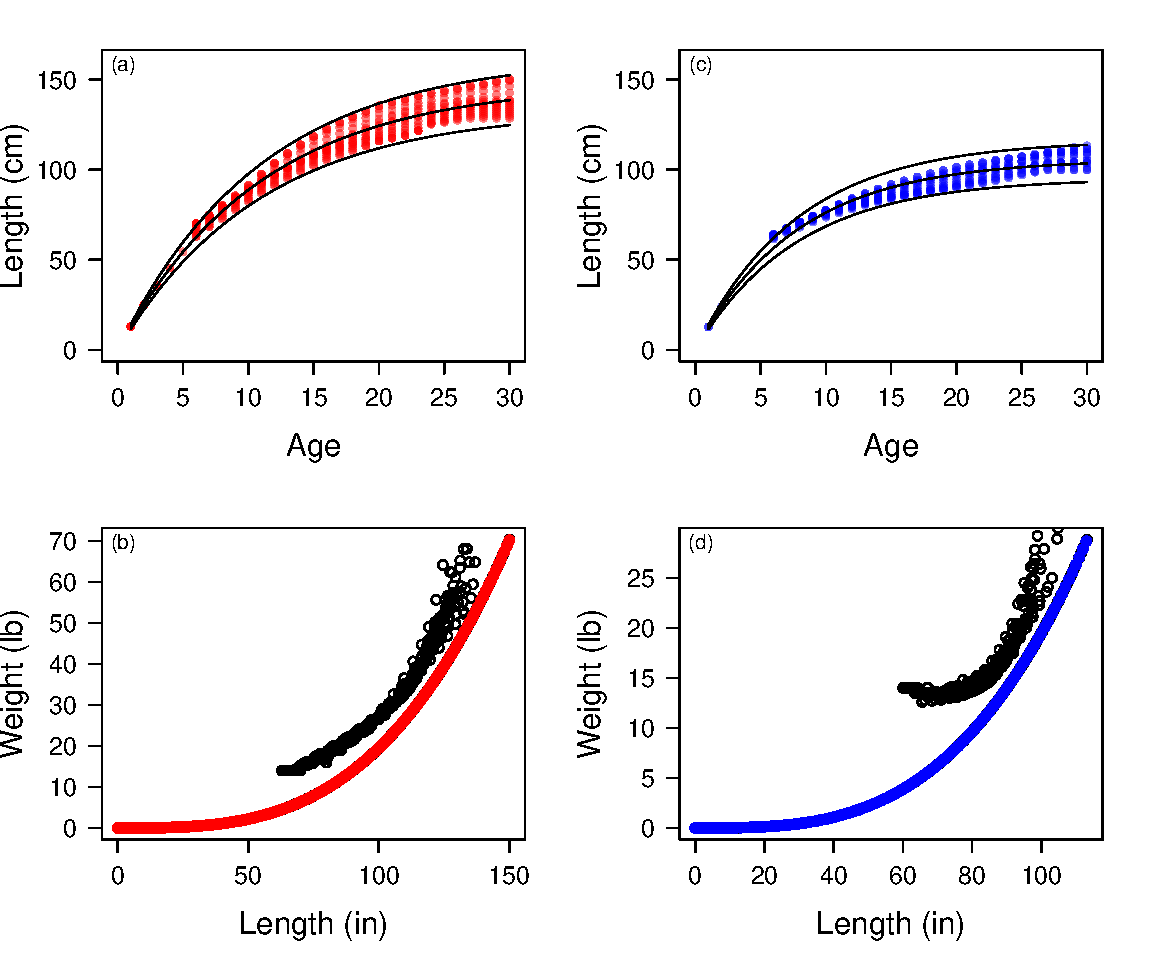
\includegraphics[width=0.9\textwidth]{../FIGURES/figLengthAtAgeFit.pdf}
	\caption{Observed mean length-at-age for female (a) and male (b) halibut in the IPHC research surveys between 1996 and 2011. Fitted lines are the von Bertalanffy growth model with the boundaries based on a 10\% coefficient of variation in the asymptotic length. Estimated parameters for females are $L_\infty=148.06$, $k=0.0915$, and for males $L_\infty=105.73$, $k=0.1275$. Panels c  (female) and d (male) show how the asymptotic length changes when cohort abundance is inversely density-dependent (solid line), density-dependent (dashed line) and density indepdent (dotted line).}
	\label{fig:FIGURES_figLengthAtAgeFit}
\end{figure}



% subsection overview_of_the_simulation_model (end)

% section simulation_model (end)